\subsection{DLR Jet-in-Hot-Coflow Burner}
%%%%%%%%%%%%%%%%%%%%%%%%%%%%%%%%%%%%%%%%%
For \href{https://develop.openfoam.com/committees/hpc/-/tree/develop/combustion/reactingFoam/LES/DLRJHC}{DLR Jet-in-Hot-Coflow Burner} testcase, 
the solution of stiff ordinary differential equations (ODEs) systems is of key importance in advanced multiphysics CFD simulations; in reactive flow simulations the fluid transport is coupled to the solution of finite-rate chemistry problems. In these scenarios, the computational effort connected to the integration of the detailed chemical kinetics ODEs systems largely contributes to limit the solver speed. A possible solution to overcome this inconvenience consists of integrating the chemical ODEs systems via an adaptive multi-block explicit solver running on a Graphical Processing Unit (GPU). The idea is to dynamically redistribute the ODE system over the resources available from the GPU architecture, while the Navier-Stokes equations are solved by a multi-core CPU algorithm. The hybrid CPU/GPU solver is expected to provide a significant speed-up in reactive calculations. The performance gain is expected to increase with large-scale mechanisms, that are characterized by large workloads.

\section*{Configuration}
\begin{figure}[h]
    \centering
%    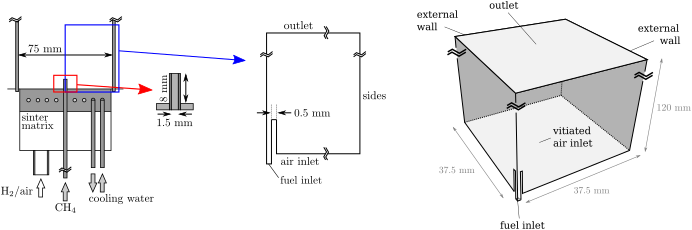
\includegraphics[width=0.6\textwidth]{figures/DLRJHC-geom.png}
    \caption{The three-dimensional geometry is based on the information available from the literature. Simplifications are introduced to account for one quarter of the entire top construction due symmetry planes.}
\end{figure}

Figure 1 (left) presents the entire structure; detailed information is reported in the literature\footnote{\url{https://doi.org/10.1080/13647830.2020.1715993}}. A pre-chamber exists below a top vessel. The top vessel is considered in the current analysis (see Fig. 2); the pre-chamber is neglected. The top of the considered chamber is open. A jet of fuel is introduced in the vessel; the region is initially filled with vitiated air coming from a preliminary combustion process between air and $H_2$ which takes place in the pre-chamber. The vitiated air is accounted as a homogeneous mixture because of the perfect mixing occurring in the pre-chamber. In the top vessel, the hot vitiated air reacts with the injected methane and generates a steady lift flame. Experiments are publicly available from the DLR Institute of Combustion Technology. 

The $L \times W \times H$ rectangular-shaped region is three-dimensional. Due to the introduced simplification, a quarter of the domain can be considered; symmetry planes are identified on two of the resulting sides. A small centered nozzle injects the fuel, while air with lean premixed hydrogen combustion products is introduced at the bottom of the mesh in the surrounding region. The walls of the fuel injector have thickness $t_w = 0.5 \, \text{mm}$. The injector diameter is $d = 2 \, \text{mm}$. The chamber has real dimensions $L \times W = 80 \, \text{mm} \times 80 \, \text{mm}$. The top is used as outlet for combustion products, thus an inlet-outlet boundary condition is applied. The temperature of the jets is $T_f = 600 \, K$ and $T_{air} = 1490 \, K$; the internal field temperature is $T_{if} = 600 \, K$. Atmospheric pressure is imposed initially. Air is used as oxidizer, but it contains a mixture of hydrogen combustion products: the mixture is composed by 72\% of $N_2$, 10\% of $O_2$, 0.2\% of $OH$, and finally 18\% of $H_2O$. The Courant number is preserved low.

\section*{Measurements}
Experiments are available from the literature for code validation\footnote{\url{https://doi.org/10.1080/13647830.2020.1715993}}.

\section*{Flow Parameters}
\begin{itemize}
    \item The fuel jet enters with high velocity: $\left| U \right| = 163.18 \, \text{m/s}$;
    \item The surrounding air (vitiated) at high temperature: $T_{air} = 1490 \, K$;
    \item Premixed lean hydrogen-air mixture from the below chamber;
    \item Premixed lean hydrogen-air mixture assumed homogeneous and reacting with methane (in top channel).
\end{itemize}

\section*{Numerical Setup}
The numerical setup is based on the DLR tutorial available in OpenFOAM-v2206. A detailed description is available on the OpenFOAM wiki\footnote{\url{https://openfoamwiki.net/index.php/Main_Page}}. The changes that allow the treatment of the considered case via GPU chemistry model are proposed subsequent sections, and include the modification of the \textit{chemistryProperties} and \textit{controlDict} files, contained in the \textit{constant} and \textit{system} folder respectively. They are consistent with the modifications proposed for the microbenchmark test case (counterFlowFlame2D). No changes are required to the numerical schemes, or to the settings of the numerical solvers. Mesh- and BC-related modifications to the problem are made to adequately treat the DLR-JHC test case.

\subsection*{Geometry and Mesh}
The problem is three-dimensional. The $L \times W \times H$ rectangular-shaped region has internal dimensions $75 \, \text{mm} \times 75 \, \text{mm} \times 120 \, \text{mm}$. The problem is reduced by considering one-quarter of the chamber; for this reason, while two external boundaries are set as walls, the remaining two are marked as symmetry planes. A single round injector of fuel is present at the center of the burner in the full construction; because of the simplification, the problem is reduced to the investigation of a quarter of the injector. Conversely to a similar tutorial available in OpenFOAM-v2206\footnote{\url{https://openfoamwiki.net/index.php/Main_Page}} (which is anyway used as starting point for the current configuration), the domain cannot be represented by means of a wedge structure: the surrounding casing (which defines the burner geometry) has a squared footprint. The mesh is generated via the \textit{blockMesh} meshing utility.

\subsection*{Models}
\begin{itemize}
    \item Solver: \textbf{reactingFoam} is used as the top-level solver.
    \item Turbulence: the problem is turbulent, hence a LES turbulence model is used.
    \item Combustion: a Partially Stirred Reactor (PaSR) combustion model is adopted.
\end{itemize}

\subsection*{Numerics}
First order, bounded, implicit time scheme; first/second order unbounded limitedLinear divergence schemes; the PIMPLE loop has 1 outer and 2 inner corrections with 0 non-orthogonal corrections. Momentum predictor is active. The fluid dynamic time step interval is initially set to $1e-6$ with an endtime of $1e-3$; the time advancement is regulated via the settings of a maxDeltaT and a maximum acceptable Courant number.

\subsection*{Boundary Conditions}
\begin{table}[H]
    \centering
    \begin{tabular}{lll}
        \hline
        Variable & Description & Units \\ \hline
        $U$ & Axial velocity & $m/s$ \\
        $p$ & Pressure & $Pa$ \\
        $T$ & Temperature & $K$ \\
        $Y_i$ & Mass fraction of the $i$-th chemical specie & - \\
        $k$ & Turbulent kinetic energy & $m^2/s^2$ \\
        $\nu_t$ & Turbulent viscosity & $m^2/s$ \\
        $\alpha_t$ & Turbulent thermal diffusivity & $kg/(m.s)$ \\ \hline
    \end{tabular}
\end{table}

\subsubsection*{Internal Field}
Pressure $p = 1e5 \, Pa$; temperature $T_{air} = 1490 \, K$; The methane concentration is 0. $Y_{N_2} = 0.7554$, $Y_{O_2} = 0.1229$, $Y_{OH} = 0.001$, and finally $Y_{H_2O} = 0.1207$. The internal field of the velocity is set to $\left| U \right| = 4.1$ along the chamber elongation (toward the outlet).

\subsubsection*{Fuel Inlet}
\begin{table}[H]
    \centering
    \begin{tabular}{lll}
        \hline
        Variable & Type & Value \\ \hline
        $U$ & fixedValue & 163.18 \\
        $p$ & zeroGradient & - \\
        $T$ & fixedValue & 600 \\
        $\alpha_t$ & calculated & 0 \\
        $\nu_t$ & calculated & 0 \\
        $k$ & fixedValue & 0.375 \\
        $Y_{O_2}$ & fixedValue & 0 \\
        $Y_{N_2}$ & fixedValue & 0 \\
        $Y_{OH}$ & fixedValue & 0 \\
        $Y_{H_2O}$ & fixedValue & 0 \\
        $Y_{CH_4}$ & fixedValue & 1 \\ \hline
    \end{tabular}
\end{table}

For $U$, the value comes from the imposition of a mass flow rate, considering a density value $\rho_{f} = 0.71682 \, kg/m^3$.

\subsubsection*{Air Inlet}
\begin{table}[H]
    \centering
    \begin{tabular}{lll}
        \hline
        Variable & Type & Value \\ \hline
        $U$ & fixedValue & 4.1 \\
        $p$ & zeroGradient & - \\
        $T$ & fixedValue & 1490 \\
        $\alpha_t$ & calculated & 0 \\
        $\nu_t$ & calculated & 0 \\
        $k$ & turbulentIntensityKineticEnergyInlet & 0.02 \\
        $Y_{O_2}$ & fixedValue & 0.1207 \\
        $Y_{N_2}$ & fixedValue & 0.7554 \\
        $Y_{OH}$ & fixedValue & 0.001 \\
        $Y_{H_2O}$ & fixedValue & 0.1229 \\
        $Y_{CH_4}$ & fixedValue & 0 \\ \hline
    \end{tabular}
\end{table}

\subsubsection*{Outlet}
\begin{table}[H]
    \centering
    \begin{tabular}{lll}
        \hline
        Variable & Type & Value \\ \hline
        $U$ & pressureInletOutletVelocity & internalField \\
        $p$ & totalPressure & internalField \\
        $T$ & inletOutlet & internalField \\
        $\alpha_t$ & calculated & internalField \\
        $\nu_t$ & calculated & internalField \\
        $k$ & inletOutlet & internalField \\
        $Y_{O_2}$ & inletOutlet & internalField \\
        $Y_{N_2}$ & inletOutlet & internalField \\
        $Y_{OH}$ & inletOutlet & internalField \\
        $Y_{H_2O}$ & inletOutlet & internalField \\
        $Y_{CH_4}$ & inletOutlet & internalField \\ \hline
    \end{tabular}
\end{table}

\section*{Validation}
The GRI-Mech 3.0 chemical chain is added to the \textit{constant} folder. A preliminary set of results is available in the \textit{validation} state. The results contained in the postProcessing folder must be consistent with those available in the \textit{validation/CPU} folder, obtained at endTime (hot simulation). The solutions are extracted along multiple axial lines across the real three-dimensional domain.

\begin{figure}[h]
    \centering
%    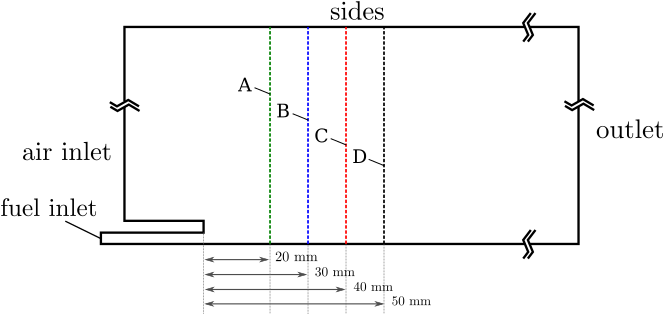
\includegraphics[width=0.8\textwidth]{figures/DLRJHC-lines.png}
    \caption{Axial lines in the geometry.}
\end{figure}

The code validation is performed by comparing the results produced by the developed run against those available in the literature.

\section*{Benchmark}
\begin{itemize}
    \item Known to run with OpenFOAM-v2206;
    \item A single folder case is provided;
    \item Multiple tests can be performed by varying the number of cells;
    \item The time taken to perform code validation and complete the simulation with the proposed setup depends on the computational hardware and the multi-core availability;
    \item Automatic light post processing for code validation via \textit{gnuplot} eases code development and debug;
    \item Heterogeneous CPU/GPU solution can be obtained by following the instruction provided for the microbenchmark counterFlowFlame2D.
\end{itemize}